\documentclass[conference]{IEEEtran}
% Relatório parcial (1ª entrega) — CIN0020 Sinais e Sistemas 2026.2
% Compilação: pdflatex entrega1.tex (duas vezes, para referências).
% As figuras referenciadas estão em ../figures/ (PDF vetorial).
\usepackage[T1]{fontenc}
\usepackage[utf8]{inputenc}
\usepackage[brazil]{babel}
\usepackage{cite}
\usepackage{amsmath,amssymb}
\usepackage{graphicx}
\usepackage{booktabs}
\usepackage{url}
\usepackage{balance}
\graphicspath{{../figures/}}

\title{Análise de sinais de vibração de drones:\\caracterização temporal e espectral de hélices saudáveis e danificadas}

\author{
\IEEEauthorblockN{Fernando Luis Campelo dos Anjos}
\IEEEauthorblockA{Centro de Informática — UFPE\\Recife, Brasil}
\and
\IEEEauthorblockN{Ludmila Cabral Lopes Magnani}
\IEEEauthorblockA{Centro de Informática — UFPE\\Recife, Brasil}
\and
\IEEEauthorblockN{Marina Rodas Sales}
\IEEEauthorblockA{Centro de Informática — UFPE\\Recife, Brasil}
}

\begin{document}
\maketitle

\begin{abstract}
Este relatório parcial analisa sinais reais de aceleração de um drone com hélices saudáveis e danificadas, do dataset DronePropB (111 registros, acelerômetro piezoelétrico a 10~kHz). Os sinais foram verificados, deduplicados e divididos em 5\,280 janelas de 1~s, das quais foram extraídas características nos domínios do tempo e da frequência. No tempo, a intensidade (RMS) é dominada pela velocidade de operação e, como indicadora de defeito, inverte de direção entre velocidades. Na frequência, os espectros são harmônicos e o dano produz assinaturas estruturais: fundamental deslocada cerca de 5\% para baixo e energia mais espalhada, com a entropia espectral maior na condição danificada em todas as velocidades (melhor separador univariado, $|d|$ médio $=0{,}74$; AUC $=0{,}71$). Demonstram-se ainda o compromisso de resolução espectral ($\Delta f = 1/T$) e o rebatimento de componentes por subamostragem sem filtro (aliasing). A análise de redundância fundamenta o conjunto de características proposto para a etapa de classificação da 2ª entrega.
\end{abstract}

\begin{IEEEkeywords}
vibração de drones, análise espectral, FFT, extração de características, detecção de falhas
\end{IEEEkeywords}

\section{Introdução}
Motores e hélices de drones produzem vibrações mecânicas cuja intensidade e composição em frequência podem ser alteradas por desgaste ou danos nas hélices, comprometendo estabilidade e segurança de voo. Este trabalho aplica conceitos de Sinais e Sistemas --- caracterização de sinais, medidas de potência, Transformada de Fourier, análise espectral e amostragem --- a dados reais de aceleração, com dois objetivos: (i) extrair e interpretar características dos sinais nos domínios do tempo e da frequência, comparando hélices saudáveis e danificadas; (ii) identificar, por separabilidade e redundância, o conjunto de características mais promissor para a classificação binária da 2ª entrega. Nenhum modelo de aprendizado de máquina é treinado nesta etapa. O código completo, executável no Google Colab, está no repositório do projeto\footnote{\url{https://github.com/marsales/Drones-Analysis}}.

\section{Dataset e preparação dos dados}

\subsection{Dataset e registros selecionados}
O DronePropB~\cite{dronepropb} contém 111 arquivos \texttt{.mat} nomeados \texttt{F\{f\}\_SV\{s\}\_SP\{v\}\_C\{c\}[\_R\{r\}]}: \texttt{F0\_SV0} indica hélice saudável e F1--F3 três tipos de falha com severidades SV1--SV3 (a documentação não especifica qual número corresponde a qual tipo de dano); SP1--SP3 são velocidades de operação (RPM não documentado), C1--C4 configurações (significado não documentado) e R1--R3 repetições (apenas nos saudáveis). Cada arquivo traz um canal de acelerômetro piezoelétrico (\texttt{AccData}, $f_s = 10$~kHz, unidade não documentada --- adotamos \emph{u.a.}) e, exceto em C4, uma IMU de 3 eixos a 1~kHz em m/s$^2$. O hardware (drone Quanser QDrone~2, hélices HQ 7$\times$4,5$''$) é descrito no artigo do dataset associado DronePropA~\cite{droneprop_a}, citado aqui apenas como contexto.

Foram selecionados os \textbf{108 registros com motor ligado} (SP1--SP3, C1--C3). As condições são comparáveis porque todos usam o mesmo drone e sensor, e toda comparação saudável $\times$ danificada é feita \emph{dentro da mesma velocidade e configuração}; as datas de aquisição mostram que a repetição R1 dos saudáveis foi gravada nos mesmos dias dos danificados. Os três registros \texttt{SP0\_C4} (motores parados) servem apenas de piso de ruído espectral. A tabela completa de registros e metadados está em \texttt{results/tabela\_registros.csv}.

\subsection{Verificação e deduplicação}
Verificou-se, registro a registro: ausência de NaN/Inf; vetor de tempo uniforme (desvio máximo de $dt$ em relação a $1/f_s$ da ordem de $10^{-14}$~s) e $f_s$ medida igual à declarada; ausência de saturação (no máximo 2 amostras no valor extremo); média $\approx 0$ no piezo ($|\mu| \le 0{,}011$~u.a.); e ausência de transientes de partida/parada (razão entre o desvio padrão do primeiro/último segundo e o global entre 0,69 e 1,25 em todos os registros) --- nenhum corte foi necessário. Duas particularidades documentadas: (i) os registros saudáveis C1 e C2 de mesma velocidade e repetição são \textbf{idênticos amostra a amostra} nos 9 pares (mesma gravação física rotulada duas vezes); cada gravação recebeu um identificador único e é contada uma só vez nas estatísticas; (ii) os saudáveis C3 das repetições R2/R3 têm 60~s, e não os 20~s nominais da configuração C3 --- as durações reais foram usadas.

\subsection{Janelamento}
Os sinais foram divididos em \textbf{janelas de 1~s} (10\,000 amostras, sem sobreposição, sobra final descartada), preservando a identificação do registro de origem: 5\,280 janelas no total; após deduplicação, 320 saudáveis e 1\,260 danificadas por velocidade (desbalanceamento $\approx 3{,}9{:}1$, relevante para a 2ª entrega). Com $N = 10^4$ e $f_s = 10$~kHz, cada janela rende $\Delta f = 1$~Hz.

\section{Análise no domínio do tempo}
A Fig.~\ref{fig:tempo} compara o par de referência (SP2, C1): \texttt{F0\_SV0\_SP2\_C1\_R1} (saudável) $\times$ \texttt{F1\_SV3\_SP2\_C1} (danificada, severidade máxima). Os sinais são oscilações de média nula moduladas em amplitude, qualitativamente parecidas nas duas condições.

\begin{figure}[htbp]
  \centering
  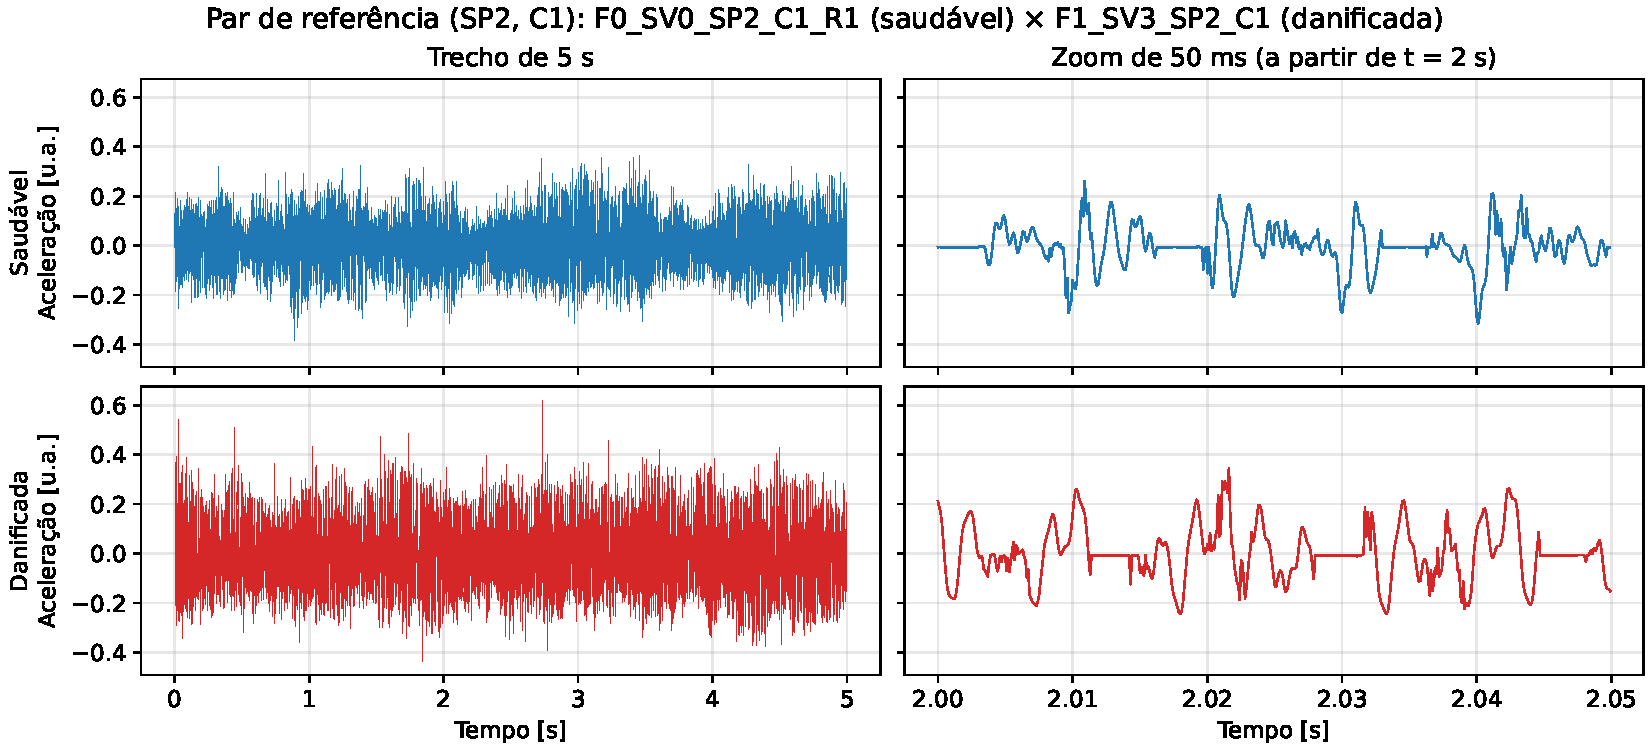
\includegraphics[width=\columnwidth]{tempo_par_referencia.pdf}
  \caption{Aceleração no tempo, par de referência (SP2, C1): trecho de 5~s e zoom de 50~ms, mesmas escalas nas duas condições.}
  \label{fig:tempo}
\end{figure}

Para cada janela bruta $x[n]$ calculamos: média $\mu$; RMS $=\sqrt{\frac{1}{N}\sum_n x[n]^2}$; potência média $P = \mathrm{RMS}^2$; desvio padrão $\sigma$ (populacional); pico absoluto $\max|x[n]|$; amplitude pico a pico; fator de crista $=\max|x[n]|/\mathrm{RMS}$; e, como extras, curtose (convenção de Pearson, $=3$ para sinal gaussiano) e assimetria. A Tabela~\ref{tab:tempo} resume as medianas e a Fig.~\ref{fig:boxplots} os boxplots por velocidade.

\begin{table}[htbp]
\caption{Medianas por condição e velocidade (janelas deduplicadas)}
\label{tab:tempo}
\centering
\small
\begin{tabular}{llccc}
\toprule
Característica & Condição & SP1 & SP2 & SP3 \\
\midrule
RMS [u.a.] & saudável & 0,039 & 0,086 & 0,207 \\
           & danificada & 0,025 & 0,092 & 0,237 \\
Pico abs. [u.a.] & saudável & 0,186 & 0,367 & 0,755 \\
           & danificada & 0,134 & 0,410 & 0,894 \\
Fator de crista & saudável & 5,10 & 4,33 & 3,56 \\
           & danificada & 5,44 & 4,38 & 3,71 \\
Curtose & saudável & 4,20 & 3,77 & 3,23 \\
           & danificada & 4,25 & 3,88 & 3,39 \\
\bottomrule
\end{tabular}
\end{table}

\begin{figure}[htbp]
  \centering
  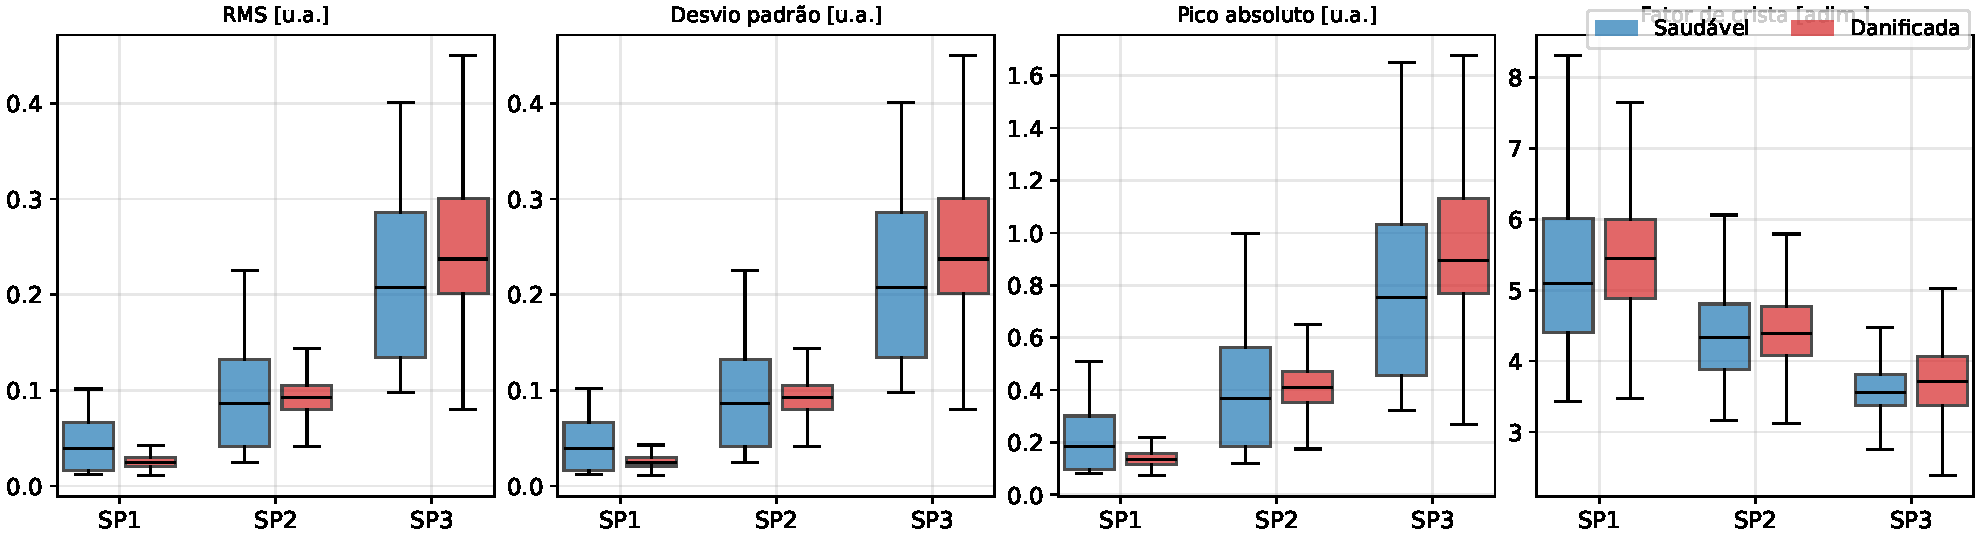
\includegraphics[width=\columnwidth]{tempo_boxplots.pdf}
  \caption{Boxplots por janela de RMS, desvio padrão, pico absoluto e fator de crista, por condição e velocidade.}
  \label{fig:boxplots}
\end{figure}

\textbf{Interpretação.} A velocidade domina a intensidade (RMS cresce quase $10\times$ de SP1 a SP3). Dentro de cada velocidade, a diferença entre condições é menor e \emph{sem direção única}: a danificada vibra mais em SP2 ($+7\%$) e SP3 ($+15\%$), porém \textbf{menos} em SP1 ($-38\%$) --- a hipótese ``defeito $\Rightarrow$ vibração mais intensa'' não se sustenta em geral. Curtose pouco acima de 3 e fator de crista decrescente com a velocidade refletem mais a velocidade que a condição. Quanto à redundância: por construção $\mathrm{RMS}^2 = P = \sigma^2 + \mu^2$; como $\mu \approx 0$ no piezo, RMS, potência e $\sigma$ carregam a mesma informação ($\rho$ de Spearman $=1{,}000$), e pico absoluto $\approx$ pico a pico$/2$ ($\rho = 0{,}996$). O efeito da componente média foi ilustrado com o eixo~Z da IMU: com $\mu \approx 9{,}72$~m/s$^2$ (gravidade), o RMS ($10{,}4$~m/s$^2$) quase triplica o $\sigma$ ($3{,}7$~m/s$^2$) --- a componente DC responde por $\approx 87\%$ da potência sem relação com vibração; RMS/potência só medem intensidade vibratória com média nula ou removida.

\section{Análise no domínio da frequência}

\subsection{FFT, normalização e espectros}
Para cada janela: remoção da média, janela de Hann $w[n]$ e FFT real, com eixo $f_k = k f_s/N$ (0 a 5\,000~Hz, $\Delta f = 1$~Hz) e espectro unilateral de amplitude $A(f_k) = 2|X(f_k)|/\sum_n w[n]$ (sem o fator 2 em DC e Nyquist), em que uma senoide de amplitude $A$ aparece com altura $\approx A$. As potências (total e por banda) usam a PSD unilateral (periodograma com Hann), integrada por trapézios. O teorema de Parseval foi verificado numericamente (erro relativo $2\times 10^{-16}$).

A Fig.~\ref{fig:espectros} mostra os espectros médios por condição e velocidade com as cinco bandas adotadas e o piso de ruído, e a Fig.~\ref{fig:zoom} o zoom na região dos picos principais.

\begin{figure}[htbp]
  \centering
  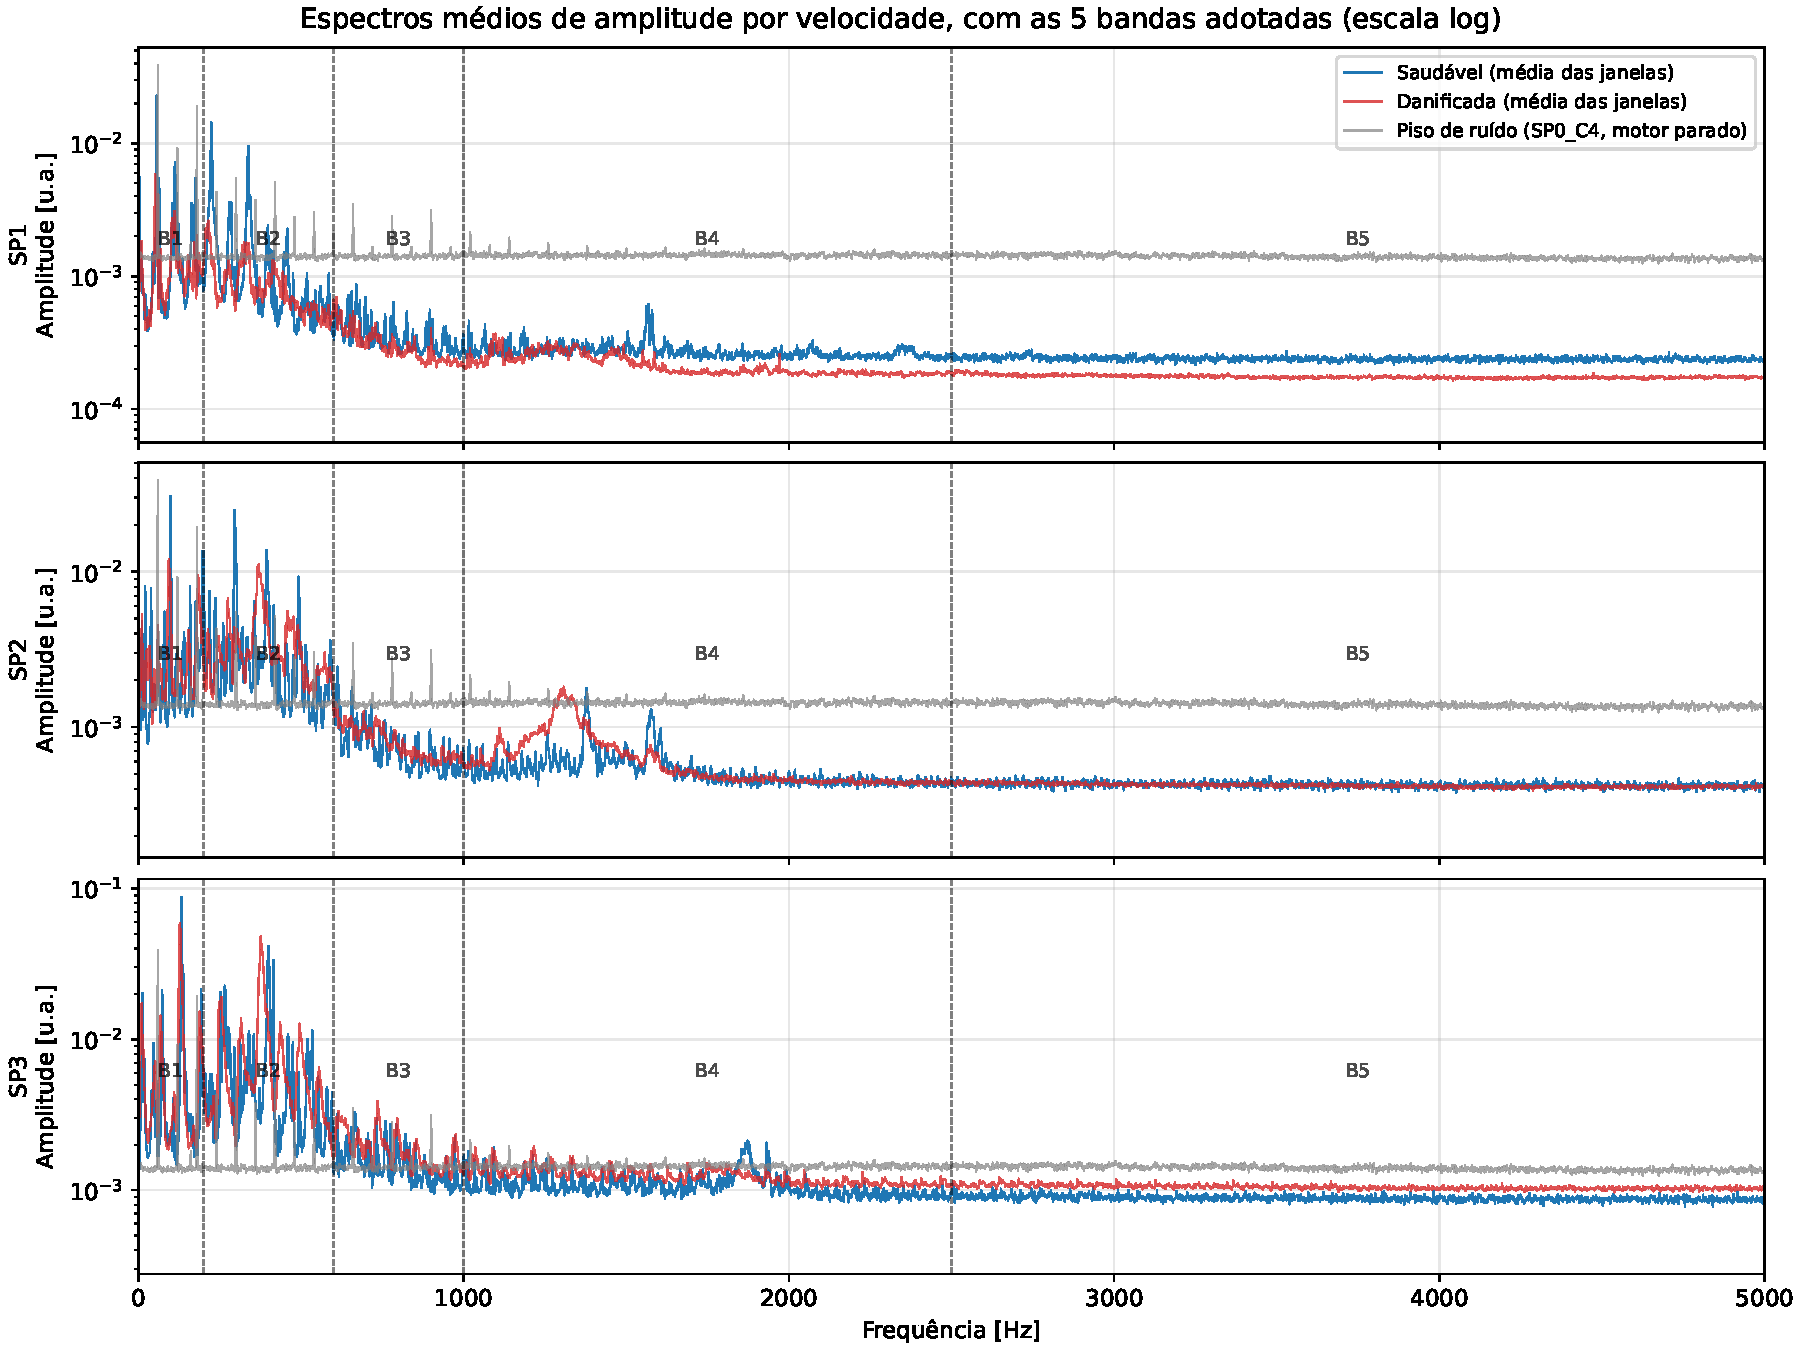
\includegraphics[width=\columnwidth]{freq_espectros_medios_bandas.pdf}
  \caption{Espectros médios de amplitude (escala log) por velocidade, com as bandas B1--B5 e o piso de ruído (\texttt{SP0\_C4}, motores parados).}
  \label{fig:espectros}
\end{figure}

\begin{figure}[htbp]
  \centering
  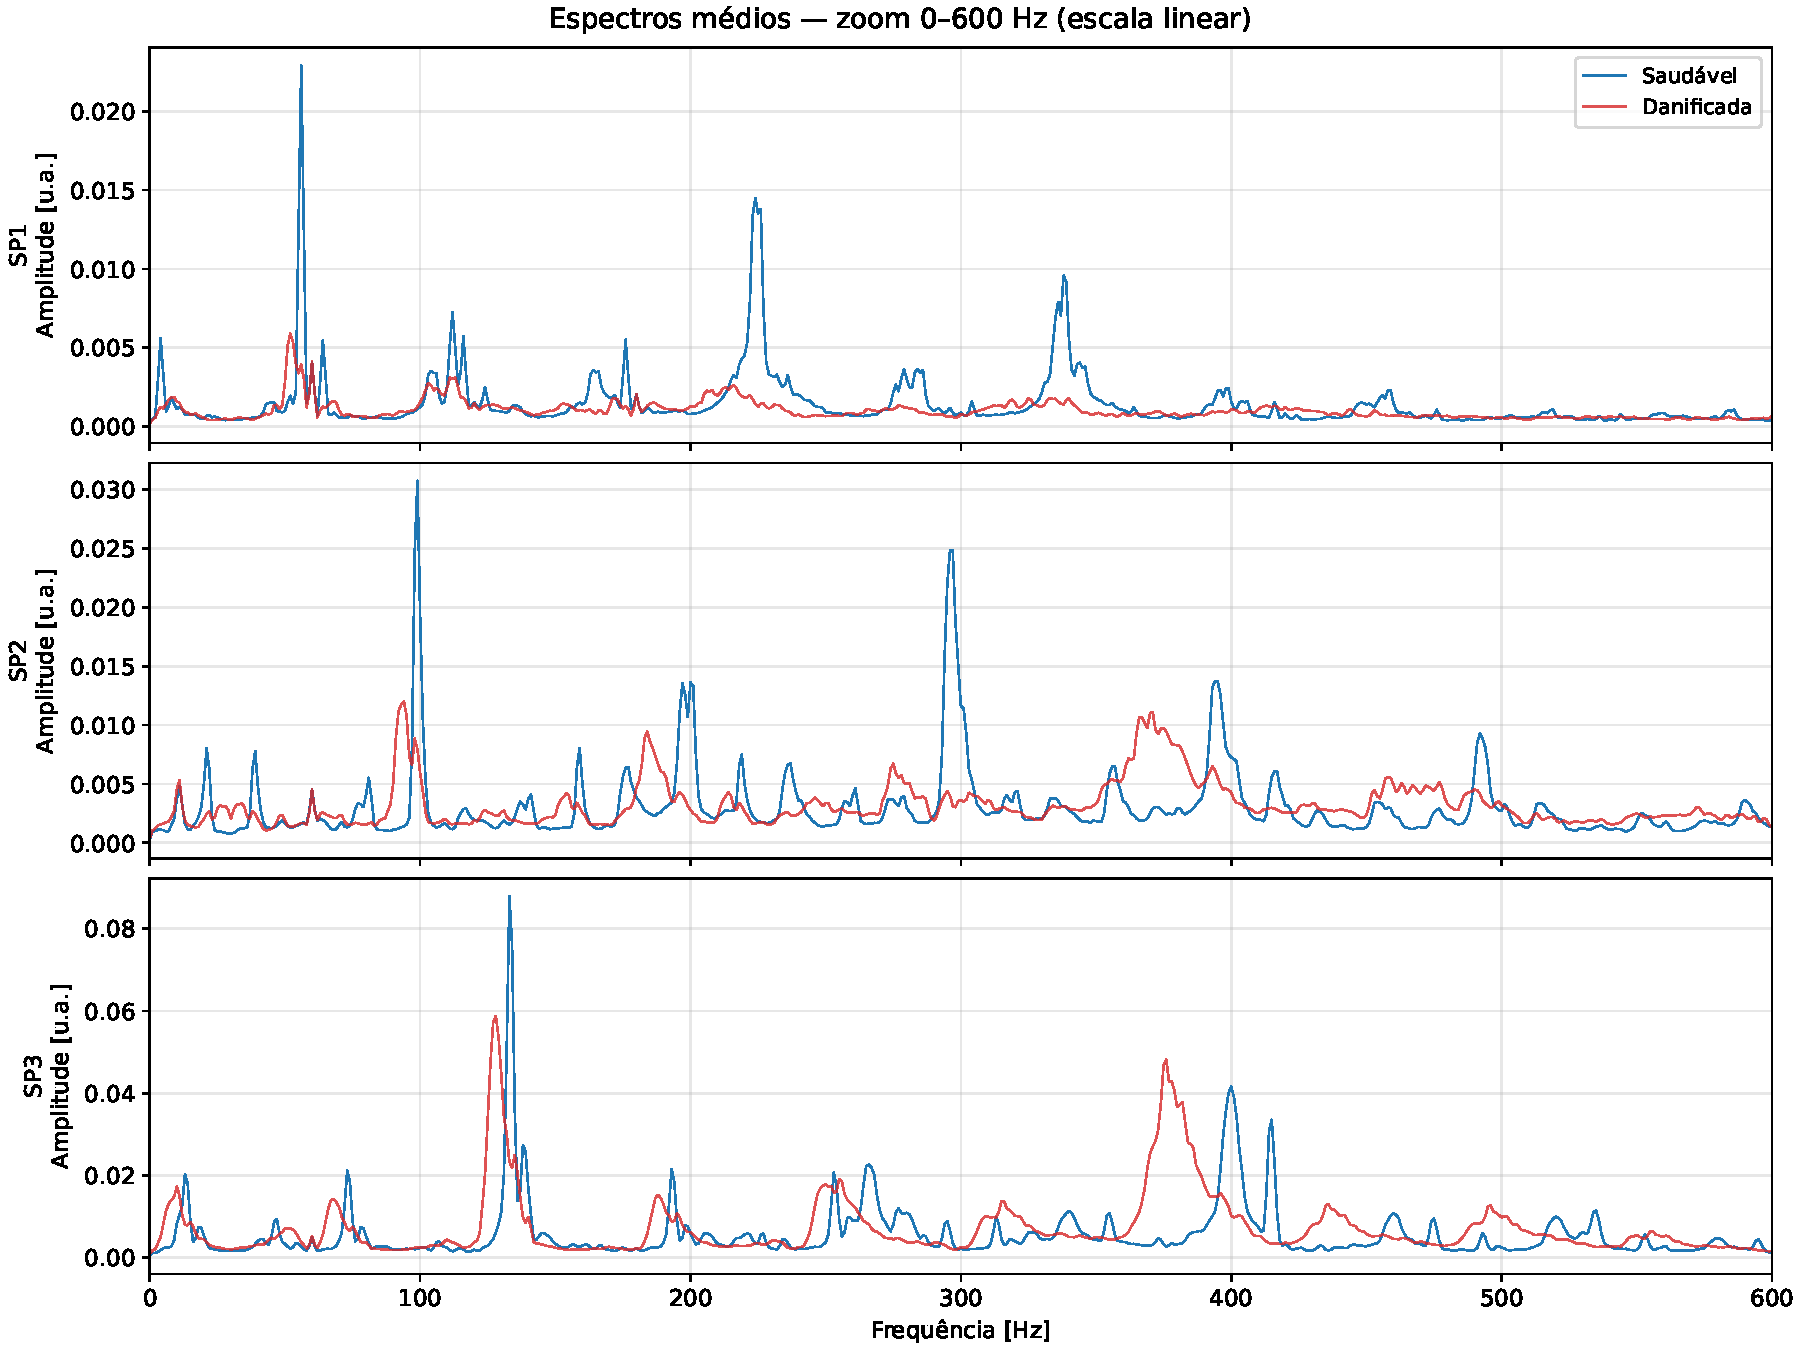
\includegraphics[width=\columnwidth]{freq_espectros_zoom600.pdf}
  \caption{Espectros médios, zoom 0--600~Hz (escala linear): estrutura harmônica e deslocamento dos picos na condição danificada.}
  \label{fig:zoom}
\end{figure}

\textbf{Leitura dos espectros.} (i) Quase todo o conteúdo está abaixo de $\sim$2\,000~Hz; o piso de ruído exibe picos em múltiplos de 60~Hz com motores parados (hipótese: interferência da rede elétrica). (ii) Os espectros com motor são \emph{harmônicos}: fundamental de $\approx 56/99/133$~Hz (saudável, SP1/SP2/SP3) com múltiplos quase exatos (SP2: razões 1,00/2,02/2,99/3,98/4,97). Como o RPM não é documentado, tratamos como hipótese que a fundamental acompanha a rotação. (iii) O dano desloca a fundamental $\approx 4$--$5\%$ para baixo (SP2: 94 $\times$ 99~Hz; SP3: 128 $\times$ 133~Hz) e cria lombadas largas próprias (ex.: $\approx 370$~Hz em SP2/SP3) onde a saudável tem picos estreitos --- diferenças de \emph{composição}, invisíveis no domínio do tempo.

\subsection{Características espectrais}
Por janela, com a mesma convenção em todas as condições: frequência dominante ($\arg\max_f A(f)$, excluindo DC); magnitude do pico dominante; potência (absoluta e fracionária) em cinco bandas; centroide espectral $\sum_k f_k S(f_k)/\sum_k S(f_k)$; e entropia espectral normalizada $-\sum_k p_k \log_2 p_k / \log_2 K$, $p_k = S(f_k)/\sum_j S(f_j)$ (0 = tom puro; 1 = ruído branco). As bandas, definidas após inspeção dos espectros médios, são B1 = 0--200~Hz (fundamental e primeiros harmônicos), B2 = 200--600~Hz (harmônicos superiores, região de maior contraste entre condições), B3 = 600--1000~Hz, B4 = 1000--2500~Hz e B5 = 2500--5000~Hz (alta frequência, próxima do piso). A Tabela~\ref{tab:freq} resume as medianas mais informativas.

\begin{table}[htbp]
\caption{Características espectrais: medianas (deduplicado)}
\label{tab:freq}
\centering
\small
\begin{tabular}{llccc}
\toprule
Característica & Condição & SP1 & SP2 & SP3 \\
\midrule
Entropia espectral & saudável & 0,53 & 0,50 & 0,37 \\
                   & danificada & 0,61 & 0,53 & 0,43 \\
Centroide [Hz] & saudável & 394 & 406 & 396 \\
               & danificada & 470 & 457 & 365 \\
Fração B2 (200--600) & saudável & 0,49 & 0,60 & 0,57 \\
                     & danificada & 0,37 & 0,64 & 0,56 \\
Fração B4 (1000--2500) & saudável & 0,033 & 0,027 & 0,019 \\
                       & danificada & 0,054 & 0,050 & 0,016 \\
\bottomrule
\end{tabular}
\end{table}

\textbf{Interpretação.} A \textbf{entropia espectral é maior na danificada em todas as velocidades}: o dano espalha a energia, reduzindo a concentração nos picos harmônicos. As frações de potência por banda diferem com direção dependente da velocidade (fração em B4 maior na danificada em SP1/SP2 e menor em SP3). A frequência dominante por janela é instável como medida contínua: harmônicos de amplitudes próximas alternam a raia vencedora entre janelas.

\subsection{Resolução espectral e aliasing}
\textbf{Resolução} (Fig.~\ref{fig:resolucao}): a FFT de trechos de 0,1~s, 1~s e 10~s do mesmo registro tem $\Delta f = f_s/N$ de 10, 1 e 0,1~Hz. Com 0,1~s os picos viram lóbulos largos e componentes separadas por menos de 10~Hz se fundem; com 10~s o pico de $\approx 296$~Hz se decompõe em componentes próximas que $\Delta f = 1$~Hz fundia. A duração escolhida (1~s) equilibra resolução e quantidade de janelas.

\begin{figure}[htbp]
  \centering
  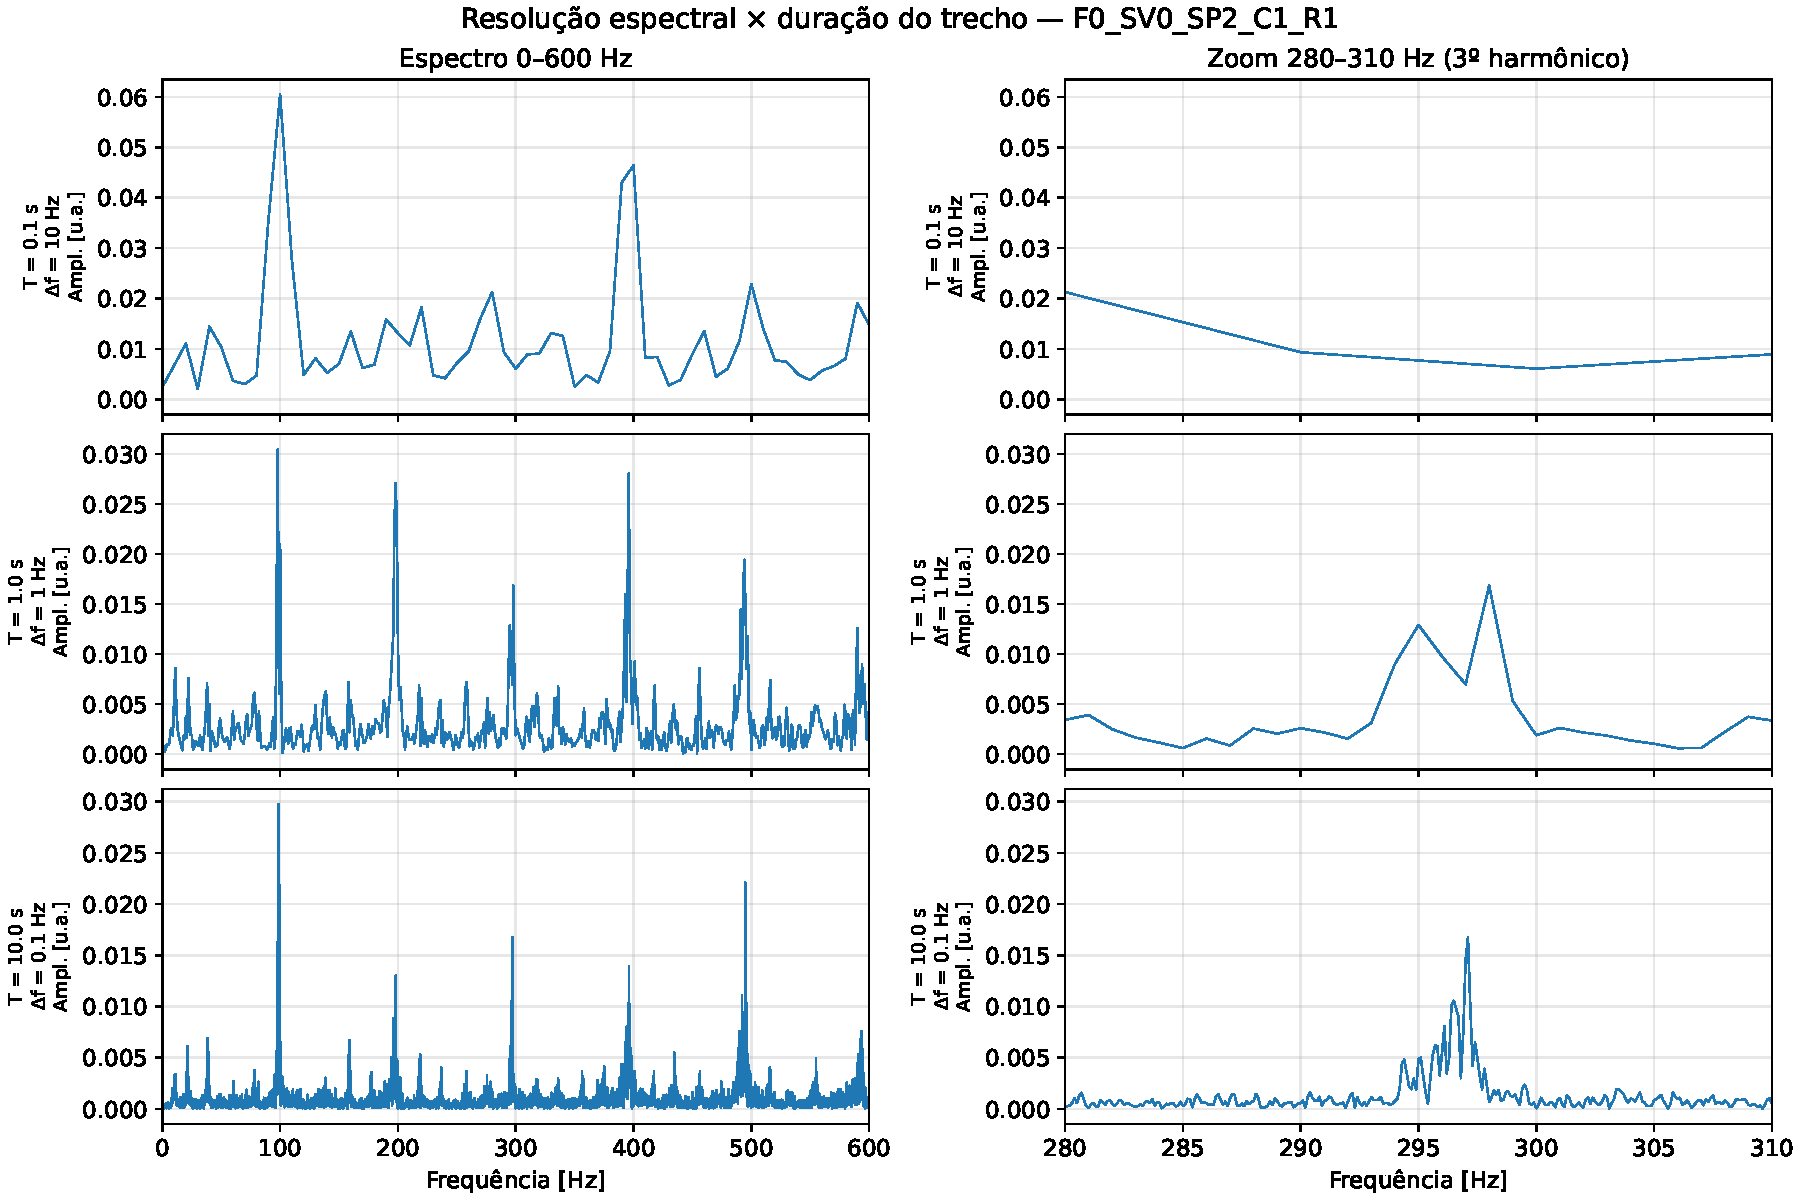
\includegraphics[width=\columnwidth]{freq_resolucao.pdf}
  \caption{Efeito da duração do trecho ($T = 0{,}1$, 1 e 10~s) sobre o espectro do mesmo registro: $\Delta f = 1/T$.}
  \label{fig:resolucao}
\end{figure}

\textbf{Aliasing} (Fig.~\ref{fig:aliasing}): um registro SP3 foi reduzido de 10~kHz para $f_s' = 500$~Hz (Nyquist $=250$~Hz) por (i) subamostragem ingênua $x[::20]$ e (ii) decimação com filtro anti-aliasing FIR. Os picos acima de 250~Hz rebatem para $f_{alias} = |f - k f_s'|$: a previsão $403{,}6 \rightarrow 96{,}4$~Hz confirmou-se (amplitude 0,091~u.a. no espectro ingênuo contra 0,001 no decimado), e $254{,}7 \rightarrow 245{,}3$~Hz; as componentes abaixo de 250~Hz permanecem nos lugares. Sem filtro, o espectro medido conteria picos em frequências incorretas, corrompendo as características espectrais.

\begin{figure}[htbp]
  \centering
  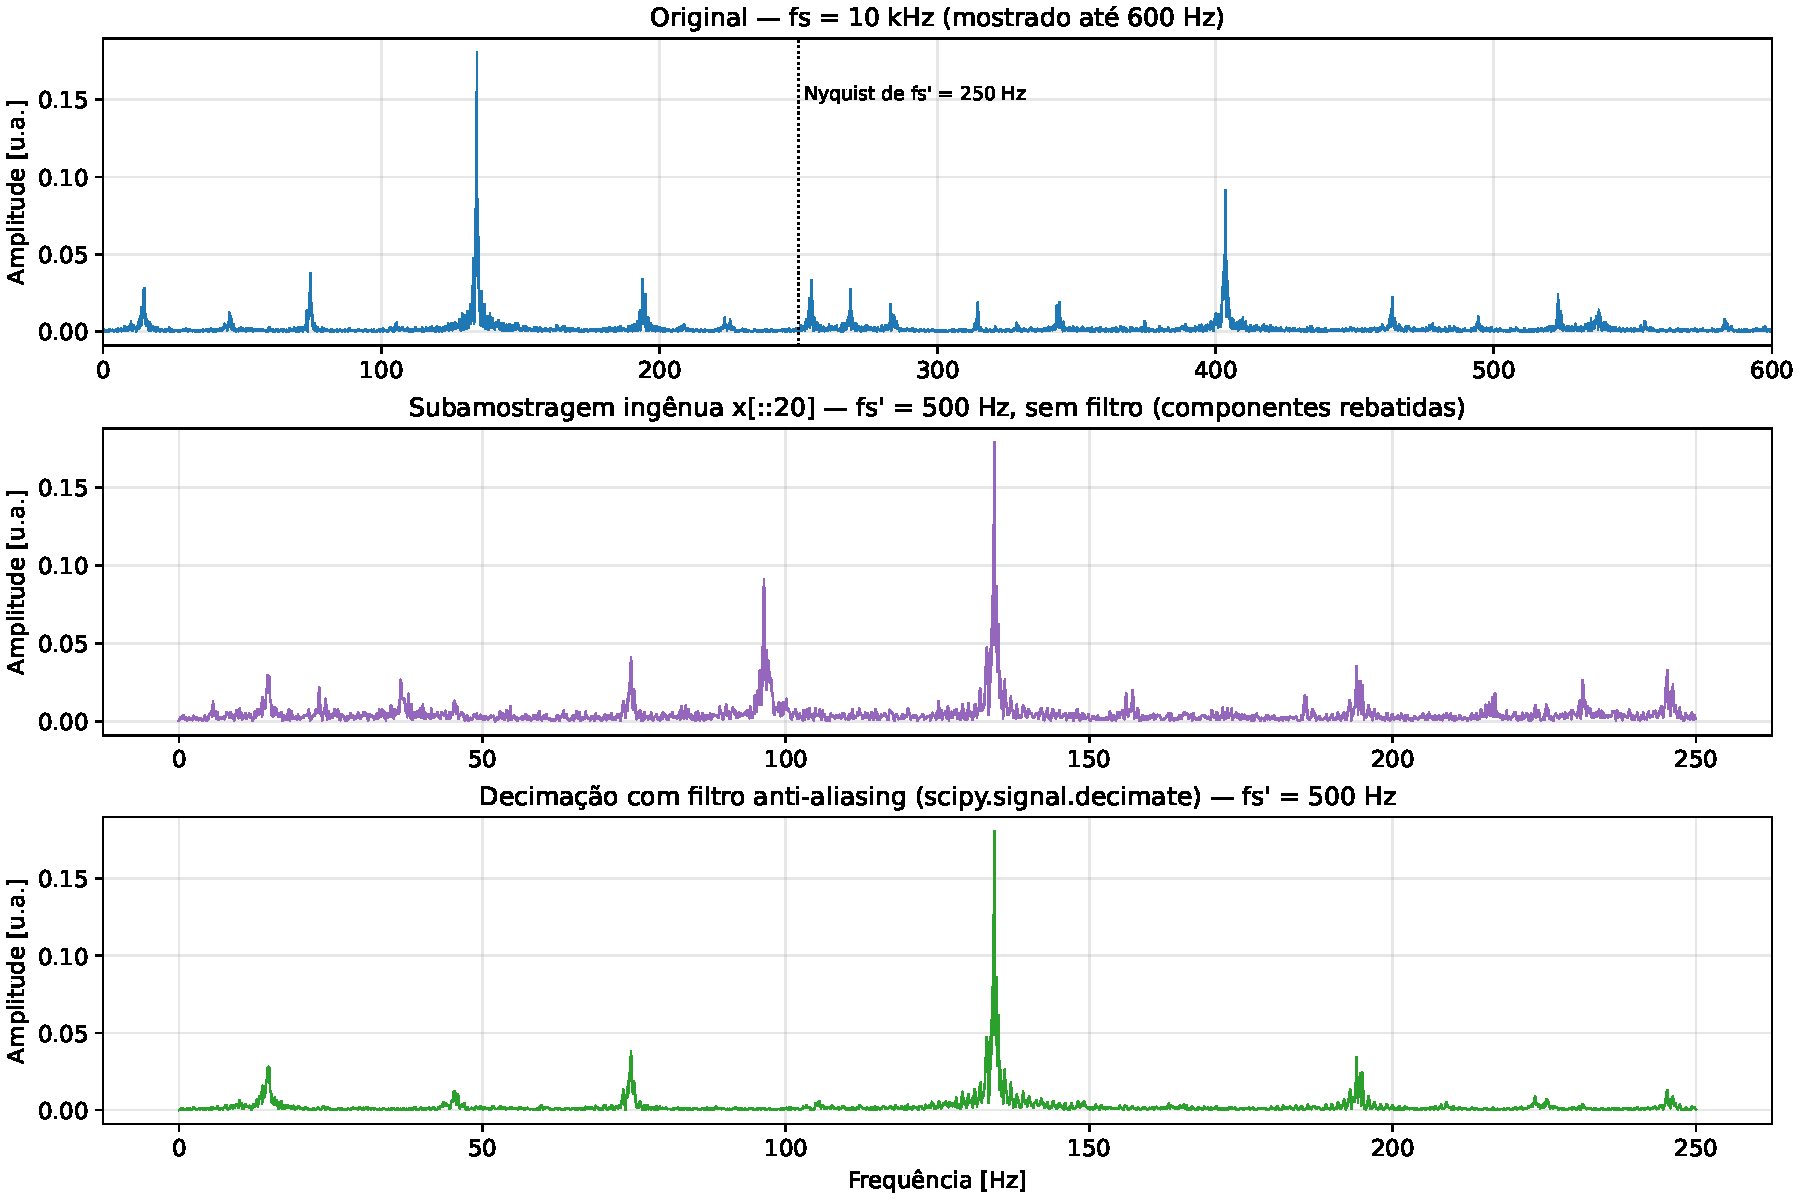
\includegraphics[width=\columnwidth]{freq_aliasing.pdf}
  \caption{Aliasing: espectro original (10~kHz), subamostragem ingênua a 500~Hz (picos rebatidos) e decimação com filtro anti-aliasing.}
  \label{fig:aliasing}
\end{figure}

\section{Comparação entre os domínios}
A separação saudável $\times$ danificada de cada característica foi quantificada por velocidade com o tamanho de efeito $|d|$ de Cohen e a AUC univariada de Mann--Whitney (sem treinar modelo; Fig.~\ref{fig:separabilidade}). Dois achados sustentados pelos dados:

\textbf{Achado 1 --- a intensidade temporal mede velocidade, não condição.} O RMS separa perfeitamente as velocidades, mas dentro de cada SP é fraco e muda de direção ($|d| = 0{,}83/0{,}28/0{,}57$ em SP1/SP2/SP3, AUC $\le 0{,}63$); um detector baseado em ``vibrou mais'' erraria sistematicamente em SP1.

\textbf{Achado 2 --- a assinatura espectral é estrutural e mais estável.} A entropia espectral é o melhor separador geral ($|d|$ médio $=0{,}74$, AUC média $=0{,}71$, direção consistente), e a fração de potência em 1000--2500~Hz atinge $|d| = 0{,}87$--$1{,}01$ (AUC $\approx 0{,}75$) em SP2/SP3 --- coerente com o deslocamento da fundamental e o espalhamento de energia dos espectros.

Nenhum domínio vence sempre: em SP1 as características de intensidade estão entre as melhores, enquanto em SP2/SP3 dominam as espectrais relativas.

\begin{figure}[htbp]
  \centering
  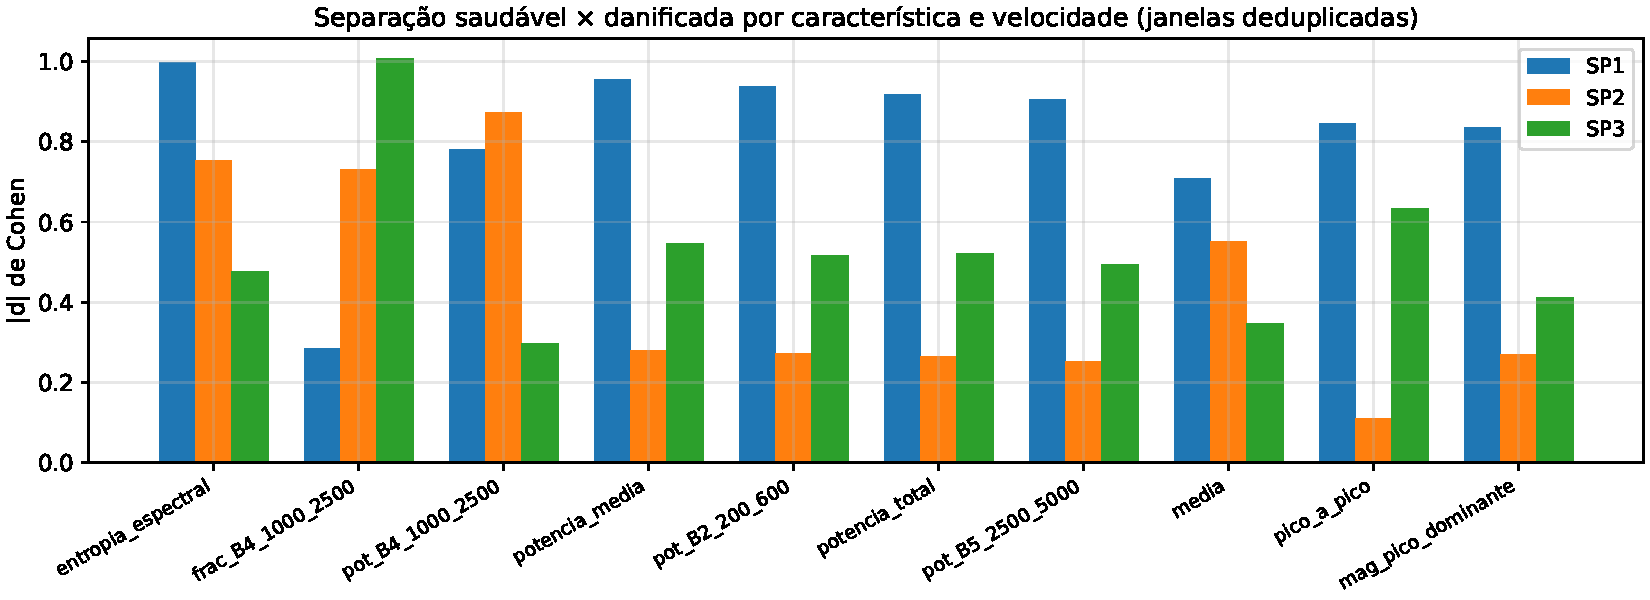
\includegraphics[width=\columnwidth]{comp_separabilidade.pdf}
  \caption{Separação saudável $\times$ danificada ($|d|$ de Cohen) das 10 melhores características, por velocidade.}
  \label{fig:separabilidade}
\end{figure}

\textbf{Redundância e conjunto proposto.} A matriz de Spearman identifica grupos intercambiáveis: \{RMS, potência, $\sigma$\} ($\rho = 1$); \{pico absoluto, pico a pico\} ($\rho = 0{,}996$); potências absolutas por banda $\times$ RMS ($\rho > 0{,}94$ --- a informação específica das bandas está nas frações). Para a classificação da 2ª entrega propõe-se: \emph{temporais} RMS, pico absoluto, fator de crista, curtose e assimetria; \emph{espectrais} entropia, centroide, frequência dominante e frações de potência em B1, B2 e B4. A média foi excluída apesar de $|d| = 0{,}55$ em SP2: num piezoelétrico ela é offset residual de condicionamento, e usá-la arriscaria aprender um artefato de aquisição.

\section{Investigação adicional}
\textbf{Pergunta:} como a velocidade de operação modifica os picos espectrais e a separação entre as condições? \textbf{Método:} picos dos espectros médios e razões harmônicas por SP; evolução da separabilidade univariada. \textbf{Resultados} (Fig.~\ref{fig:fundamental}): a fundamental cresce de forma aproximadamente proporcional à velocidade (saudável: $56 \rightarrow 99 \rightarrow 133$~Hz; danificada: $52 \rightarrow 94 \rightarrow 128$~Hz) mantendo a estrutura harmônica, e a razão entre as fundamentais das duas condições é estável ($\approx 0{,}95$): \textbf{o dano reduz a frequência de rotação efetiva em $\approx 5\%$ em todas as velocidades} (efeito registrado sem afirmar o mecanismo, pois o RPM não é documentado). A separação não melhora monotonicamente com a velocidade: cada SP tem seu melhor separador ($|d|$ máximo $\approx 1{,}0/0{,}87/1{,}0$), e o $|d|$ médio das 5 melhores características é similar ($\approx 0{,}9/0{,}7/0{,}7$) --- a velocidade muda \emph{quais} características separam, mais do que \emph{quanto}; convém treinar com registros de todas as velocidades.

\begin{figure}[htbp]
  \centering
  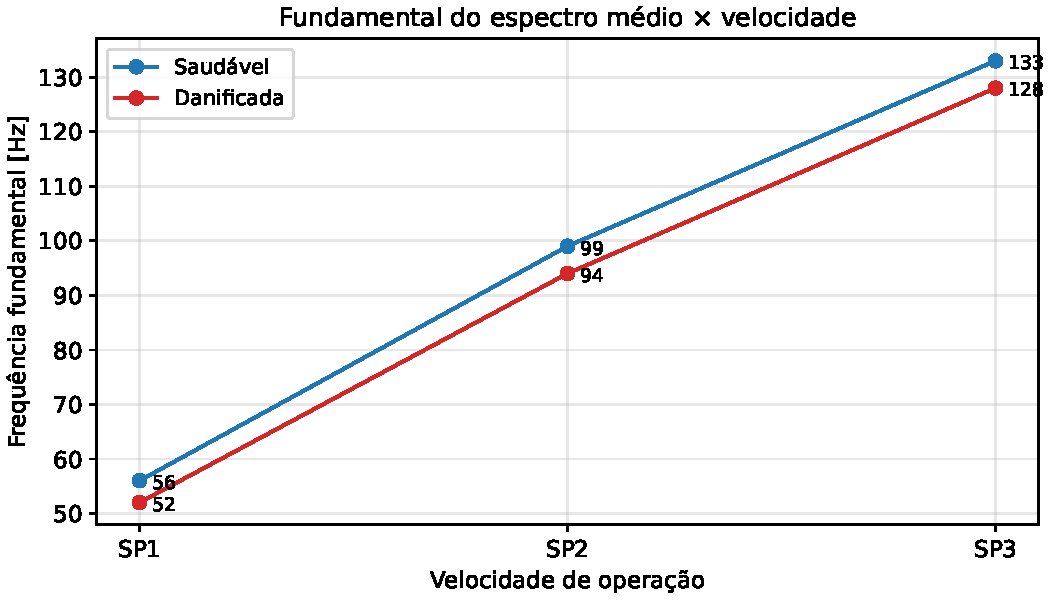
\includegraphics[width=0.85\columnwidth]{invest_fundamental_sp.pdf}
  \caption{Frequência fundamental do espectro médio por velocidade e condição.}
  \label{fig:fundamental}
\end{figure}

\section{Conclusões}
Os dados do DronePropB mostraram-se íntegros e comparáveis após verificação, deduplicação das cópias C1/C2 saudáveis e janelamento em 1~s (5\,280 janelas, 23 características). No tempo, a intensidade é dominada pela velocidade e é indicadora ambígua de defeito; na frequência, o dano deixa assinaturas estruturais consistentes (fundamental $\approx 5\%$ mais baixa, energia mais espalhada, entropia espectral maior em todas as velocidades). Limitações: unidade do piezo, configurações C e RPM não documentados; desbalanceamento $\approx 3{,}9{:}1$; uma única gravação por condição danificada, o que impede separar completamente efeito da condição e da sessão de aquisição. A tabela de características por janela e o conjunto proposto deixam a classificação pronta para a 2ª entrega, que deverá separar treino/teste por registro e tratar o desbalanceamento.

\balance
\begin{thebibliography}{2}
\bibitem{dronepropb}
M.~A.~A. Ismail, M.~E. Elshaar, A.~Abdalla e Q.~Quan, ``DronePropB: ground testing dataset for commercial drones with defective propellers,'' \emph{Mendeley Data}, V1, 2024. DOI: 10.17632/xkvfjmm8zg.1.

\bibitem{droneprop_a}
M.~A.~A. Ismail \emph{et al.}, ``DronePropA: ground testing dataset for commercial drones,'' \emph{Data in Brief}, 2025. DOI: 10.1016/j.dib.2025.111589.
\end{thebibliography}

\end{document}
